\section{Productivity, Output and Employment}

The output of an economy depends on (1) the quantities of inputs (labor, capital, raw materials) and (2) the productivity of inputs.

\subsection{The production function}

The textbook / FNCE 1018 develops a two-factor model of production. 

\begin{definition}
    The \textbf{production function} states that 
    \[
        Y = AF(K, N)
    \]
    where
    \begin{align*}
        Y &= \text{ real output produced in a given period of time} \\
        A &= \text{total factor productivity} \\
        K &= \text{ capital stock} \\
        N &= \text{ labor, or number of workers} \\
        F &= \text{ some function relating $Y$ to $K, N$}
    \end{align*}
\end{definition}

\begin{example}
    The \textbf{Cobb-Douglas} production function states that 
    \[
        Y = AK^{a} N^{1-a}
    \]
    Empirically,
    \[
        Y = AK^{0.3} N^{0.7}
    \]
\end{example}
% --- Remarks and plot for Y as a function of K (N constant) ---
\begin{remarks}
    Under Cobb-Douglas, holding $N$ constant and varying $K$:
    \begin{itemize}
        \item $Y$ increases with $K$, but at a decreasing rate (diminishing marginal product of capital).
    \end{itemize}
    and vice versa. \\
    \begin{minipage}{0.48\textwidth}
    \begin{center}
        \begin{tikzpicture}
            \begin{axis}[
                    scale = 0.7,
                    xmin = 0, xmax = 10,
                    ymin = 0, ymax = 10,
                    axis lines* = left, 
                    xtick = {0}, ytick = \empty,
                    clip = false,
                ]
                % Y = AK^{0.3}N^{0.7}, with A=3, N=2
                \addplot[
                    domain = 0:10,
                    restrict y to domain = 0:10,
                    samples = 800,
                    color = black,
                ]{3*x^0.3*2^0.7};
                \node[right] at (current axis.right of origin) {$K$};
                \node[above] at (current axis.above origin) {$Y$};
            \end{axis}
        \end{tikzpicture} 
        \\
        \textbf{Fig - $Y$ as a function of $K$, fixed $N$}
    \end{center}
    \end{minipage}%
    \hfill
    \begin{minipage}{0.48\textwidth}
    \begin{center}
    \begin{tikzpicture}
        \begin{axis}[
                scale = 0.7,
                xmin = 0, xmax = 10,
                ymin = 0, ymax = 10,
                axis lines* = left, 
                xtick = {0}, ytick = \empty,
                clip = false,
            ]
            % Y = AK^{0.3}N^{0.7}, with A=3, K=2
            \addplot[
                domain = 0:10,
                restrict y to domain = 0:10,
                samples = 800,
                color = black,
            ]{3*x^0.3*2^0.7};
            \node[right] at (current axis.right of origin) {$N$};
            \node[above] at (current axis.above origin) {$Y$};
        \end{axis}
    \end{tikzpicture}
    \\
    \textbf{Fig - $Y$ as a function of $K$, fixed $N$}
    \end{center}
    \end{minipage}
\end{remarks}

\begin{definition}
    The \textbf{Marginal product of capital} is the increase in output produced that results from a one-unit increase in capital stock. 
    \[
        MPK = \frac{\triangle Y}{\triangle K}
    \]
\end{definition}

\begin{definition}
    The \textbf{Marginal product of labor} is the increase in output produced that results from a one-unit increase in labor. 
    \[
        MPN = \frac{\triangle Y}{\triangle N}
    \]
\end{definition}

\begin{remarks}
    The $MPK$ and $MPN$
    \begin{itemize}
        \item are positive 
        \item are decreasing in $K$ / $N$, due to diminishing marginal product
    \end{itemize} 
\end{remarks}

\subsection{Adverse productivity shock}

\begin{remarks}
Given a decrease in $A$, 
    \begin{itemize}
        \item the marginal product decreases for every value of $N$
        \item the amount of output decreases for every value of $N$
    \end{itemize} 
    \begin{minipage}{\textwidth}
    
    \centering
    \begin{tikzpicture}
        \begin{axis}[
                scale = 0.7,
                xmin = 0, xmax = 10,
                ymin = 0, ymax = 10,
                axis lines* = left, 
                xtick = {0}, ytick = \empty,
                clip = false,
            ]
            % Y = AK^{0.3}N^{0.7}, with A=3, K=2
            \addplot[
                domain = 0:10,
                restrict y to domain = 0:10,
                samples = 800,
                color = black,
            ]{3*x^0.3*2^0.7};
            \addplot[
                domain = 0:10,
                restrict y to domain = 0:10,
                samples = 800,
                color = red,
            ]{1.5*x^0.3*2^0.7};
            \node[right] at (current axis.right of origin) {Labor, $N$};
            \node[above] at (current axis.above origin) {Output, $Y$};
            \node[right] at (10, 3 * 10^0.3 * 2^0.7) {$Y_1 = A_1K^{\alpha} N^{1-\alpha}$};
            \node[right] at (10, 1.5 * 10^0.3 * 2^0.7) {$Y_2 = A_2K^{\alpha} N^{1-\alpha}$};
        \end{axis}
    \end{tikzpicture}
    \\
    \textbf{Fig - Decrease in $A$, holding $K$ fixed}
    \end{minipage}

    Note that 
    \begin{align*}
        &A_2 < A_1 \\
        \implies&  Y_2 < Y_1 \\
        \implies&  MPN_2 = A_2 K^{\alpha} {(1-\alpha) N^{-\alpha}} < A_1 K^{\alpha} (1 - \alpha) N^{-\alpha} = MPN_1
    \end{align*}
\end{remarks}

\subsection{Labor Demand}

Assumptions for the labor market model:
\begin{itemize}
    \item all workers alike
    \item firms view wages as being determined by competitive labor market
    \item firms aim to maximize profits
\end{itemize} 

The marginal product of labor measures the benefit of employing additional worker in terms of extra output produced. 

\begin{definition}
    \textbf{Marginal revenue product of labor} is the benefit of employing an additioinal worker in terms of the extra revenue produced. 
    \[
        MRPN = P \times MPN
    \]
\end{definition}

The quantity of labor demanded is 
\begin{itemize}
    \item in nominal terms: equal to the $MRPN$
    \item in real terms: equal to $MPN$
\end{itemize} 

\begin{definition}
    \text{Real wage} refers to the wage measured in terms of units of output.
    \[
        w = \frac{W}{P}
    \]
\end{definition}

\begin{remarks}
    Note that firms will want to increase employment under the following condition, all 4 statements are equivalent
    \begin{align*}
        & MPN > w  \\
        \iff & MPN > \frac{W}{P}  \\
        \iff & P \times MPN > W  \\
        \iff & MPRN > W 
    \end{align*}

    Vice versa for condition under which the firm will want to decrease employment
\end{remarks}

\begin{remarks}
    For a single firm, the wage is set by the market 
    \begin{center}
    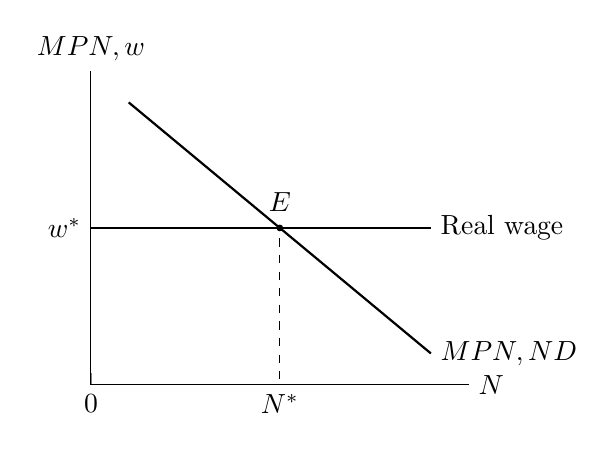
\begin{tikzpicture}
        \begin{axis}[
        scale = 0.7,
        xmin = 0, xmax = 10,
        ymin = 0, ymax = 10,
        axis lines* = left,
        xtick = {0}, ytick = \empty,
        clip = false,
        ]
        % Supply and demand curves
        \addplot[color = black, thick] coordinates {(1, 9) (9, 1)};
        \addplot[color = black, thick] coordinates {(0, 5) (9, 5)};
        % Dashed lines
        \addplot[color = black, dashed] coordinates {(0, 5) (5, 5) (5, 0)};
        % Coordinate points
        \addplot[color = black, mark = *, only marks, mark size = 1pt]
        coordinates {(5, 5)};
        % Labels
        \node [right] at (current axis.right of origin) {$N$};
        \node [above] at (current axis.above origin) {$MPN, w$};
        \node [above] at (5, 5.2) {$E$};
        \node [left] at (0, 5) {$w^*$};
        \node [below] at (5, 0) {$N^*$};
        \node [right] at (9, 1) {$MPN, ND$};
        \node [right] at (9, 5) {Real wage};
        \end{axis}
    \end{tikzpicture}
\end{center}
\end{remarks}

\begin{remark} 
    The following intercepts are mathematically equivalent. \\

    % -------- LEFT: real wage condition --------
    \begin{minipage}{0.48\textwidth}
    \centering
    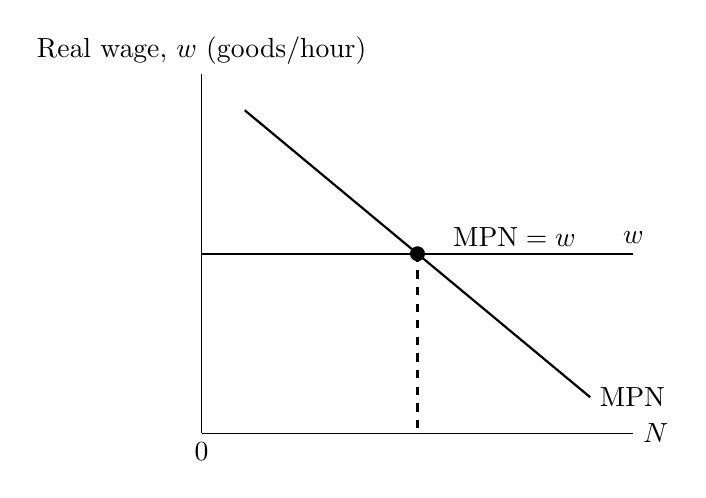
\begin{tikzpicture}
    \begin{axis}[
    scale=0.8,
    xmin=0, xmax=10,
    ymin=0, ymax=10,
    axis lines* = left,
    xtick={0}, ytick=\empty,
    clip=false,
    ]
    % MPN (downward sloping)
    \addplot[color=black, thick] coordinates {(1,9) (9,1)};
    % real wage (horizontal)
    \addplot[color=black, thick] coordinates {(0,5) (10,5)};
    % guides + point
    \addplot[color=black, dashed, thick] coordinates {(0,5) (5, 5) (5,0)};
    \addplot[color=black, mark=*, only marks, mark size=2.5pt] coordinates {(5,5)};
    % labels
    \node[right] at (current axis.right of origin) {$N$};
    \node[above] at (current axis.above origin) {Real wage, $w$ (goods/hour)};
    \node[right] at (9,1) {$\mathrm{MPN}$};
    \node[above] at (10,5) {$w$};
    \node[below right] at (5.6,6) {$\mathrm{MPN}=w$};
    \end{axis}
    \end{tikzpicture}
    \end{minipage}
    \hfill
    % -------- RIGHT: nominal/value condition --------
    \begin{minipage}{0.48\textwidth}
    \centering
    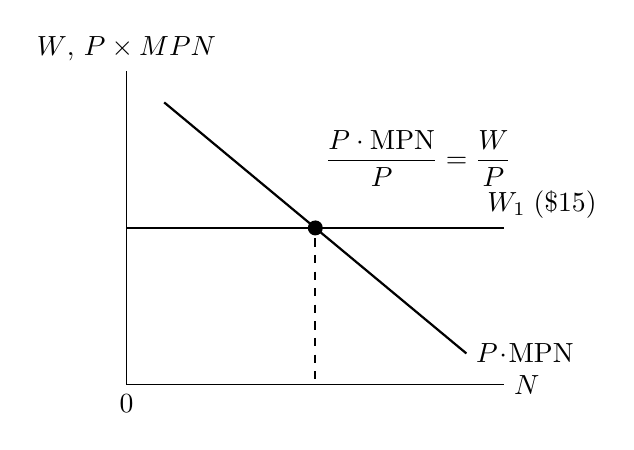
\begin{tikzpicture}
    \begin{axis}[
    scale=0.7,
    xmin=0, xmax=10,
    ymin=0, ymax=10,
    axis lines* = left,
    xtick={0}, ytick=\empty,
    clip=false,
    ]
    % P*MPN (downward sloping)
    \addplot[color=black, thick] coordinates {(1,9) (9,1)};
    % nominal wage W1
    \addplot[color=black, thick] coordinates {(0,5) (10,5)};
    % guides + point
    \addplot[color=black, dashed, thick] coordinates {(0,5) (5,5) (5,0)};
    \addplot[color=black, mark=*, only marks, mark size=2.5pt] coordinates {(5,5)};
    % labels
    \node[right] at (current axis.right of origin) {$N$};
    \node[above] at (current axis.above origin) {$W$, $P \times MPN$};
    \node[right] at (9,1) {$P\!\cdot\!\mathrm{MPN}$};
    \node[above] at (11,5) {$W_1\;(\$15)$};
    \node[above right] at (5,6) {$\displaystyle \frac{P\cdot \mathrm{MPN}}{P}=\frac{W}{P}$};
    \end{axis}
    \end{tikzpicture}
    \end{minipage}
\end{remark}


\subsubsection{Factors that shift labor demand}
\begin{remark}
Factors that affect labor demand must change the amount of labor that firms want to employ \textit{at any given level of the real wage}.\\

The labor demand increases in response to 
\begin{itemize}
    \item $A \uparrow$, productivity improvements / positive supply shock
    \item $K \uparrow$, increase in capital supply
\end{itemize} 

\begin{center}
    \begin{tikzpicture}
        \begin{axis}[
        scale = 0.7,
        xmin = 0, xmax = 10,
        ymin = 0, ymax = 10,
        axis lines* = left,
        xtick = {0}, ytick = \empty,
        clip = false,
        ]
        % Supply and demand curves
        \addplot[color = black, thick] coordinates {(1, 9) (9, 1)};
        \addplot[color = black, thick] coordinates {(3, 9) (10, 2)};

        % Labels
        \node [right] at (current axis.right of origin) {$N$};
        \node [above] at (current axis.above origin) {$MPN, w$};
        \node [right] at (9, 1) {$MPN_1$};
        \node [right] at (10, 2) {$MPN_2$};

        \draw[-{Triangle[length = 2mm, width = 1mm]}, black]
        (1.2, 9) to (2.8, 9);
        \end{axis}
    \end{tikzpicture}
\end{center}
\end{remark}

\subsubsection{Aggregate labor demand}

\begin{definition}
    \textbf{Aggregate labor demand} is the sum of labor demands of all the firms in an economy. 
\end{definition}

\begin{remark} 
    The aggregate labor demand looks the same as individual firm labor demand.
\end{remark}

\subsection{Labor supply}

\begin{definition}
    The \textbf{aggregate labor supply} is the sum of labor supplied by everyone in the economy.
\end{definition}

\subsubsection{Income-leisure trade-off and real wages}

The marginal benefit of work is the utility gained from extra income. The marginal cost of work is the utility lost from reducing leisure. 

\begin{definition}
    An individual worker seeks to maximize his or her utility function
    \[
    \max_{N} U(\mathcal{L}, \mathcal{C})
    \]
    subject to 
    \[
        \mathcal{C} = w(T - \mathcal{L}) + Z
    \]
    Where 
    \begin{align*}
        T &= \text{ total number of hours available} \\
        Z &= \text{ non-labor income} \\
        w &= \text{ real wage rate} \\
        U &= \text{ utility function with inputs $\mathcal{L}, \mathcal{C}$} \\
        \mathcal{C} &= \text{ consumption} \\
        \mathcal{L} &= T - N = \text{ leisure }
    \end{align*}
\end{definition}

\begin{definition}
    The \textbf{substitution effect} refers to an increase in the opportunity cost of leisure causing workers to substitute away from leisure towards work.
\end{definition}

\begin{remark}
    \textbf{Pure substitution effect}: one-day rise in real wage, $NS \uparrow$.  \\
\end{remark}

\begin{definition}
    The \textbf{income effect} refers to workers being better off and hence working less.
\end{definition}
\begin{remark}
    \textbf{Pure income effect}: changes in $Z$, e.g. winning the lottery, or higher expected future real wages, $NS \downarrow$ \\
\end{remark}


\begin{remark} 
    \textbf{Income} and \textbf{substition} effect work in opposite directions on labor supply.  \\

    An increase in real wages 
    \begin{itemize}
        \item raises the marginal benefit of work, increases labor supply, by \textbf{substitution effect}
        \item increases workers' wealth, decreases labor supply, by \textbf{income effect}
    \end{itemize}   
\end{remark}


\begin{remark}
    Empirically, labor supply 
    \begin{itemize}
        \item rises when there is a \textbf{temporary increase in real wage}
        \item falls when there is a \textbf{permanent increase in real wage}
    \end{itemize} 

    In aggregate, the labor supply is \textbf{rising in real wages}.

\begin{center}
    \begin{tikzpicture}
        \begin{axis}[
        scale = 0.7,
        xmin = 0, xmax = 10,
        ymin = 0, ymax = 10,
        axis lines* = left,
        xtick = {0}, ytick = \empty,
        clip = false,
        ]
        % Labor supply
        \addplot[color = black, thick] coordinates {(4, 1) (6, 10)};

        % Labels
        \node [right] at (current axis.right of origin) {$N$};
        \node [above] at (current axis.above origin) {$w$};
        \node [right] at (5, 10) {$NS$};
        \end{axis}
    \end{tikzpicture}
\end{center}
\end{remark}

\subsubsection{Factors that affect labor supply}
\begin{remark}
The labor supply shifts left in response to 
\begin{itemize}
    \item increases in weath, $NS \downarrow$
    \item increases in expected future real wage, $NS \downarrow$
    \item decrease in working age population
    \item decrease in participation rate
\end{itemize} 

\begin{center}
    \begin{tikzpicture}
        \begin{axis}[
        scale = 0.7,
        xmin = 0, xmax = 10,
        ymin = 0, ymax = 10,
        axis lines* = left,
        xtick = {0}, ytick = \empty,
        clip = false,
        ]
        % Supply and demand curves
        \addplot[color = black, thick] coordinates {(4, 1) (6, 10)};
        \addplot[color = black, thick] coordinates {(2, 1) (4, 10)};

        % Labels
        \node [right] at (current axis.right of origin) {$N$};
        \node [above] at (current axis.above origin) {$MPN, w$};
        \node [right] at (6, 10) {$NS_1$};
        \node [right] at (4, 10) {$NS_2$};
        \end{axis}
    \end{tikzpicture}
\end{center}
\end{remark}

\subsection{Labor Market Equilibrium}

Under classical assumptions, real wage adjusts reasonably quickly to bring labor demand and supply into equilibrium.


\begin{definition}
    \textbf{Full-employment level of employment}, $ \bar{N} $ is defined as the equilibrium level of employment. The corresponding market-clearing real wage is $ \bar{w} $.
\end{definition}
\begin{center}
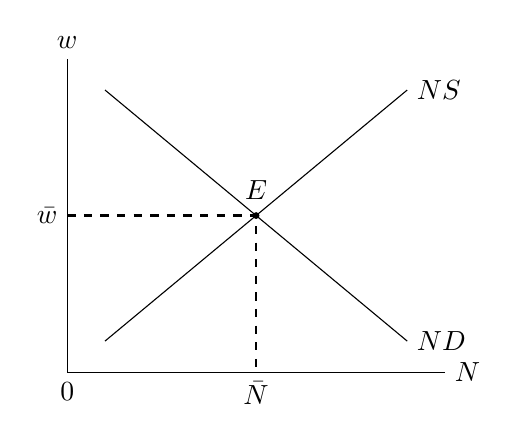
\begin{tikzpicture}
\begin{axis}[
scale = 0.7,
xmin = 0, xmax = 10,
ymin = 0, ymax = 10,
axis lines* = left,
xtick = {0}, ytick = \empty,
clip = false,
]
% Supply and demand curves
\addplot[color = black] coordinates {(1, 9) (9, 1)};
\addplot[color = black] coordinates {(1, 1) (9, 9)};
% Dashed lines
\addplot[color = black, dashed, thick] coordinates {(0, 5) (5, 5)
(5, 0)};
% Coordinate points
\addplot[color = black, mark = *, only marks, mark size = 1pt]
coordinates {(5, 5)};
% Labels
\node [right] at (current axis.right of origin) {$N$};
\node [above] at (current axis.above origin) {$w$};
\node [above] at (5, 5.2) {$E$};
\node [left] at (0, 5) {$ \bar{w}  $};
\node [below] at (5, 0) {$ \bar{N} $};
\node [right] at (9, 1) {$ND$};
\node [right] at (9, 9) {$NS$};
\end{axis}
\end{tikzpicture}
\end{center}
\subsubsection{Full employment output}
\begin{definition}
    \textbf{Full-employment output}, $\bar{Y}$, also called \textbf{potential output}, is the level of output that firms in the economy supply when wages and prices have fully adjusted. 

    $\bar{Y} $ is achieved when aggregate employment reaches its full-employment level, $\bar{N}$
    \[
        \bar{Y}  = AF \left( K, \bar{N}  \right) 
    \]
\end{definition}
\begin{remark}
    A decrease in $A$ reduces $\bar{Y} $ in two ways
    \begin{itemize}
        \item  $A \downarrow \rightarrow \bar{Y} \downarrow$ directly 
        \item  $A \downarrow \rightarrow MPN \downarrow \rightarrow ND \downarrow \rightarrow \bar{N} \downarrow \rightarrow \bar{Y} \downarrow $ 
    \end{itemize} 
\end{remark}

\subsection{Unemployment}

Under classical assumptions, all workers who are willing to work at the prevailing wage find jobs. 

\begin{remark}
    The Bureau of Labor Statistics surveys 60,000 households monthly. Each person over 16 is assigned to 
    \begin{itemize}
        \item $E$, employed, if person worked full-time or part-time during the past week
        \item $U$, unemployed, if person didn't work during the past week but looked for work in the past four weeks
        \item $NLF$, not in labor force, if the person didnt work and didn't look for work in the past 4 weeks
        \begin{itemize}
            \item discouraged workers, people who become discouraged and move from $U$ to $NLF$
        \end{itemize} 
    \end{itemize} 
    \begin{align*}
        \text{labor force} &= LF =  E + U \\
        \text{adult population} &= LF + NLF \\
        \text{participation rate} &= \frac{LF}{LF + NLF} \\
        \text{employment ratio} &= \frac{E}{LF + NLF}
    \end{align*}
\end{remark}

\begin{remark}
    US unemployment is characterized by two contradictory statements
    \begin{itemize}
        \item most unemployment spells are short ( < 2 months)
        \item most unemployed are experiencing unemployment spells with a long duration
    \end{itemize} 
\end{remark}

\begin{remark}
    Sources of unemployment 
    \begin{itemize}
        \item \textbf{frictional unemployment}: arises as workers search for suitable jobs and firms search for suitable workers
        \item \textbf{structural unemployment}: long-term and chronic unemployment that exists even when the economy is not in a recession
        \begin{itemize}
            \item unskilled, low skilled workers
            \item rellocation of labor from shrinking industries / depressed regions
        \end{itemize} 
    \end{itemize} 
\end{remark}

\begin{definition}
    The \textbf{natural rate of unemployment}, $ \bar{u} $ is the rate of unemployment that prevails when output and employment are at the full-employment level. \\

    The difference betwen actual unemployment and natural unemployment is \textbf{cyclical unemployment} 
    \[
    \text{cyclical unemployment}= u - \bar{u} 
    \]
\end{definition}

\subsection{Okun's Law}
\begin{theorem}
    \textbf{Okun's Law} states that the gap between full-employment output and actual output increases by 2 percent for each percent increase in unemployment 
    \[
    \frac{\bar{Y} - Y }{\bar{Y} } = 2 \left( u  - \bar{u}  \right) 
    \]

    Alternatively, the percentage change in real output is roughly 3 percent minus two times the change in unemployment
    \[
    \frac{\triangle Y}{Y} = \frac{\triangle \bar{Y} }{ \bar{Y} }  - 2 \triangle u
    \]
\end{theorem}

\begin{proof}
    \begin{align*}
        \frac{\bar{Y} - Y }{ \bar{Y} } &= 1 - \frac{Y}{ \bar{Y} } = c( u - \bar{u} ) \\
        \frac{Y}{ \bar{Y} } - 1= c ( \bar{u}  - u )
    \end{align*}

    Taking percentage change on both sides, we get 
    \begin{align*}
        \triangle \left( \frac{Y}{\bar{Y} } \right)  &= c \left( \triangle \bar{u} - \triangle{u} \right)  \\ 
        \frac{Y + \triangle Y}{\bar{Y}  + \triangle \bar{Y} } - \frac{Y}{ \bar{Y} } &= c \left( \triangle \bar{u}  - \triangle u \right)  \\
        \frac{\bar{Y} \triangle Y - Y \triangle \bar{Y}  }{ \bar{Y}  ( \bar{Y}  + \triangle \bar{Y} )} &= c \left( \triangle \bar{u}  - \triangle u \right) 
    \end{align*}
    Multiplying by  $ \left( \frac{\bar{Y}  + \triangle \bar{Y} }{Y} \right) \approx 1 $, 
    \begin{align*}
        \frac{\bar{Y} \triangle Y - Y \triangle \bar{Y}  }{ \bar{Y}Y} &\approx c \left( \triangle \bar{u}  - \triangle u \right)  \\
        \frac{\triangle Y}{Y} - \frac{\triangle \bar{Y} }{\bar{Y} } &\approx c \left( \triangle \bar{u}  - \triangle u \right)  \\
        \frac{\triangle Y}{Y} & \approx \frac{\triangle \bar{Y} }{ \bar{Y} } + c \left( \triangle \bar{u}  - \triangle u  \right) 
    \end{align*}

    Taking $c$ to be 2 and $\triangle \bar{u} $ to be 0, we get
    \[
    \frac{\triangle Y}{Y} = \frac{\triangle \bar{Y} }{ \bar{Y} }  - 2 \triangle u
    \]
\end{proof}


\newpage


















